\documentclass[twoside]{book}

% Packages required by doxygen
\usepackage{fixltx2e}
\usepackage{calc}
\usepackage{doxygen}
\usepackage[export]{adjustbox} % also loads graphicx
\usepackage{graphicx}
\usepackage[utf8]{inputenc}
\usepackage{makeidx}
\usepackage{multicol}
\usepackage{multirow}
\PassOptionsToPackage{warn}{textcomp}
\usepackage{textcomp}
\usepackage[nointegrals]{wasysym}
\usepackage[table]{xcolor}

% Font selection
\usepackage[T1]{fontenc}
\usepackage[scaled=.90]{helvet}
\usepackage{courier}
\usepackage{amssymb}
\usepackage{sectsty}
\renewcommand{\familydefault}{\sfdefault}
\allsectionsfont{%
  \fontseries{bc}\selectfont%
  \color{darkgray}%
}
\renewcommand{\DoxyLabelFont}{%
  \fontseries{bc}\selectfont%
  \color{darkgray}%
}
\newcommand{\+}{\discretionary{\mbox{\scriptsize$\hookleftarrow$}}{}{}}

% Page & text layout
\usepackage{geometry}
\geometry{%
  a4paper,%
  top=2.5cm,%
  bottom=2.5cm,%
  left=2.5cm,%
  right=2.5cm%
}
\tolerance=750
\hfuzz=15pt
\hbadness=750
\setlength{\emergencystretch}{15pt}
\setlength{\parindent}{0cm}
\setlength{\parskip}{0.2cm}
\makeatletter
\renewcommand{\paragraph}{%
  \@startsection{paragraph}{4}{0ex}{-1.0ex}{1.0ex}{%
    \normalfont\normalsize\bfseries\SS@parafont%
  }%
}
\renewcommand{\subparagraph}{%
  \@startsection{subparagraph}{5}{0ex}{-1.0ex}{1.0ex}{%
    \normalfont\normalsize\bfseries\SS@subparafont%
  }%
}
\makeatother

% Headers & footers
\usepackage{fancyhdr}
\pagestyle{fancyplain}
\fancyhead[LE]{\fancyplain{}{\bfseries\thepage}}
\fancyhead[CE]{\fancyplain{}{}}
\fancyhead[RE]{\fancyplain{}{\bfseries\leftmark}}
\fancyhead[LO]{\fancyplain{}{\bfseries\rightmark}}
\fancyhead[CO]{\fancyplain{}{}}
\fancyhead[RO]{\fancyplain{}{\bfseries\thepage}}
\fancyfoot[LE]{\fancyplain{}{}}
\fancyfoot[CE]{\fancyplain{}{}}
\fancyfoot[RE]{\fancyplain{}{\bfseries\scriptsize Generated on Mon Nov 16 2015 23\+:39\+:42 for seng330a2 by Doxygen }}
\fancyfoot[LO]{\fancyplain{}{\bfseries\scriptsize Generated on Mon Nov 16 2015 23\+:39\+:42 for seng330a2 by Doxygen }}
\fancyfoot[CO]{\fancyplain{}{}}
\fancyfoot[RO]{\fancyplain{}{}}
\renewcommand{\footrulewidth}{0.4pt}
\renewcommand{\chaptermark}[1]{%
  \markboth{#1}{}%
}
\renewcommand{\sectionmark}[1]{%
  \markright{\thesection\ #1}%
}

% Indices & bibliography
\usepackage{natbib}
\usepackage[titles]{tocloft}
\setcounter{tocdepth}{3}
\setcounter{secnumdepth}{5}
\makeindex

% Hyperlinks (required, but should be loaded last)
\usepackage{ifpdf}
\ifpdf
  \usepackage[pdftex,pagebackref=true]{hyperref}
\else
  \usepackage[ps2pdf,pagebackref=true]{hyperref}
\fi
\hypersetup{%
  colorlinks=true,%
  linkcolor=blue,%
  citecolor=blue,%
  unicode%
}

% Custom commands
\newcommand{\clearemptydoublepage}{%
  \newpage{\pagestyle{empty}\cleardoublepage}%
}


%===== C O N T E N T S =====

\begin{document}

% Titlepage & ToC
\hypersetup{pageanchor=false,
             bookmarks=true,
             bookmarksnumbered=true,
             pdfencoding=unicode
            }
\pagenumbering{roman}
\begin{titlepage}
\vspace*{7cm}
\begin{center}%
{\Large seng330a2 }\\
\vspace*{1cm}
{\large Generated by Doxygen 1.8.10}\\
\vspace*{0.5cm}
{\small Mon Nov 16 2015 23:39:42}\\
\end{center}
\end{titlepage}
\clearemptydoublepage
\tableofcontents
\clearemptydoublepage
\pagenumbering{arabic}
\hypersetup{pageanchor=true}

%--- Begin generated contents ---
\chapter{Hierarchical Index}
\section{Class Hierarchy}
This inheritance list is sorted roughly, but not completely, alphabetically\+:\begin{DoxyCompactList}
\item \contentsline{section}{Factory}{\pageref{class_factory}}{}
\item \contentsline{section}{Game\+Entity}{\pageref{class_game_entity}}{}
\begin{DoxyCompactList}
\item \contentsline{section}{Item}{\pageref{class_item}}{}
\item \contentsline{section}{Room}{\pageref{class_room}}{}
\end{DoxyCompactList}
\end{DoxyCompactList}

\chapter{Class Index}
\section{Class List}
Here are the classes, structs, unions and interfaces with brief descriptions\+:\begin{DoxyCompactList}
\item\contentsline{section}{\hyperlink{class_factory}{Factory} }{\pageref{class_factory}}{}
\item\contentsline{section}{\hyperlink{class_game_entity}{Game\+Entity} }{\pageref{class_game_entity}}{}
\item\contentsline{section}{\hyperlink{class_item}{Item} }{\pageref{class_item}}{}
\item\contentsline{section}{\hyperlink{class_room}{Room} }{\pageref{class_room}}{}
\end{DoxyCompactList}

\chapter{Class Documentation}
\hypertarget{class_factory}{}\section{Factory Class Reference}
\label{class_factory}\index{Factory@{Factory}}
\subsection*{Static Public Member Functions}
\begin{DoxyCompactItemize}
\item 
\hypertarget{class_factory_a96c2bf28ba98e5072521ea43be8efd02}{}static \hyperlink{class_game_entity}{Game\+Entity} $\ast$ {\bfseries make\+\_\+game\+\_\+entity} (int user\+\_\+input)\label{class_factory_a96c2bf28ba98e5072521ea43be8efd02}

\end{DoxyCompactItemize}


The documentation for this class was generated from the following files\+:\begin{DoxyCompactItemize}
\item 
/\+Users/\+Christina\+G/\+C\+S\+C/seng330/project/temp/temp2/Factory.\+h\item 
/\+Users/\+Christina\+G/\+C\+S\+C/seng330/project/temp/temp2/Game\+Entity.\+cpp\end{DoxyCompactItemize}

\hypertarget{class_game_entity}{}\section{Game\+Entity Class Reference}
\label{class_game_entity}\index{Game\+Entity@{Game\+Entity}}
Inheritance diagram for Game\+Entity\+:\begin{figure}[H]
\begin{center}
\leavevmode
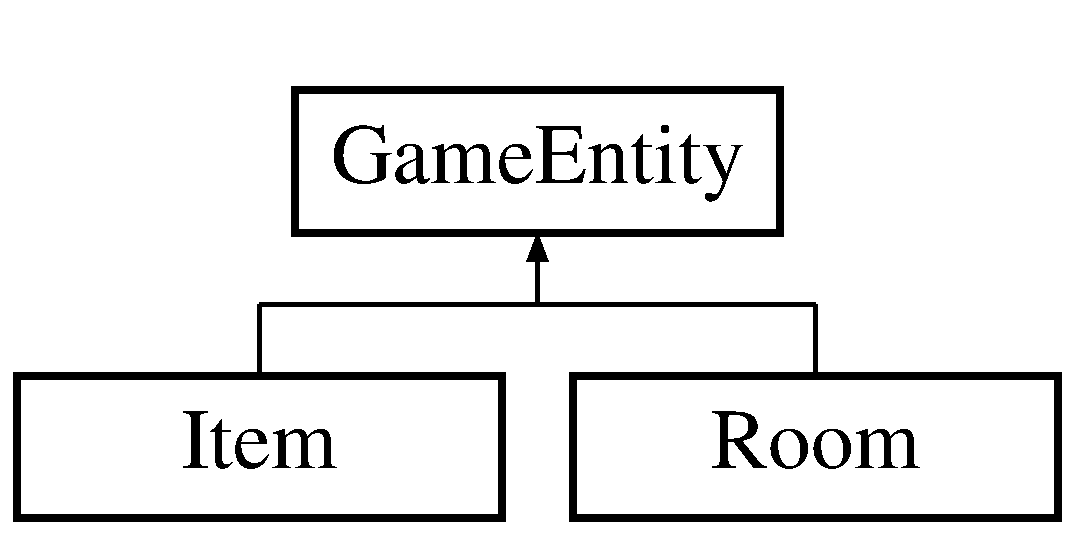
\includegraphics[height=2.000000cm]{class_game_entity}
\end{center}
\end{figure}
\subsection*{Public Member Functions}
\begin{DoxyCompactItemize}
\item 
\hypertarget{class_game_entity_ac534073fe3e7b25d95029c8af622a88e}{}{\bfseries Game\+Entity} (int id, std\+::string name)\label{class_game_entity_ac534073fe3e7b25d95029c8af622a88e}

\item 
\hypertarget{class_game_entity_a941b5c3c653f7526545bd81816e9531a}{}{\bfseries Game\+Entity} (int id, std\+::string name, std\+::string description)\label{class_game_entity_a941b5c3c653f7526545bd81816e9531a}

\item 
\hypertarget{class_game_entity_a0effae7533a6e242c71a5ccd2bb5a030}{}virtual \hyperlink{class_game_entity}{Game\+Entity} $\ast$ {\bfseries Clone} ()=0\label{class_game_entity_a0effae7533a6e242c71a5ccd2bb5a030}

\item 
\hypertarget{class_game_entity_ac909a518389ee9bc92562b4166340766}{}void {\bfseries Print} ()\label{class_game_entity_ac909a518389ee9bc92562b4166340766}

\item 
\hypertarget{class_game_entity_a163f5785614921a65aab161491d8c47c}{}void {\bfseries Set\+Description} (std\+::string description)\label{class_game_entity_a163f5785614921a65aab161491d8c47c}

\end{DoxyCompactItemize}


The documentation for this class was generated from the following files\+:\begin{DoxyCompactItemize}
\item 
/\+Users/\+Christina\+G/\+C\+S\+C/seng330/project/temp/temp2/Game\+Entity.\+h\item 
/\+Users/\+Christina\+G/\+C\+S\+C/seng330/project/temp/temp2/Game\+Entity.\+cpp\end{DoxyCompactItemize}

\hypertarget{class_item}{}\section{Item Class Reference}
\label{class_item}\index{Item@{Item}}
Inheritance diagram for Item\+:\begin{figure}[H]
\begin{center}
\leavevmode
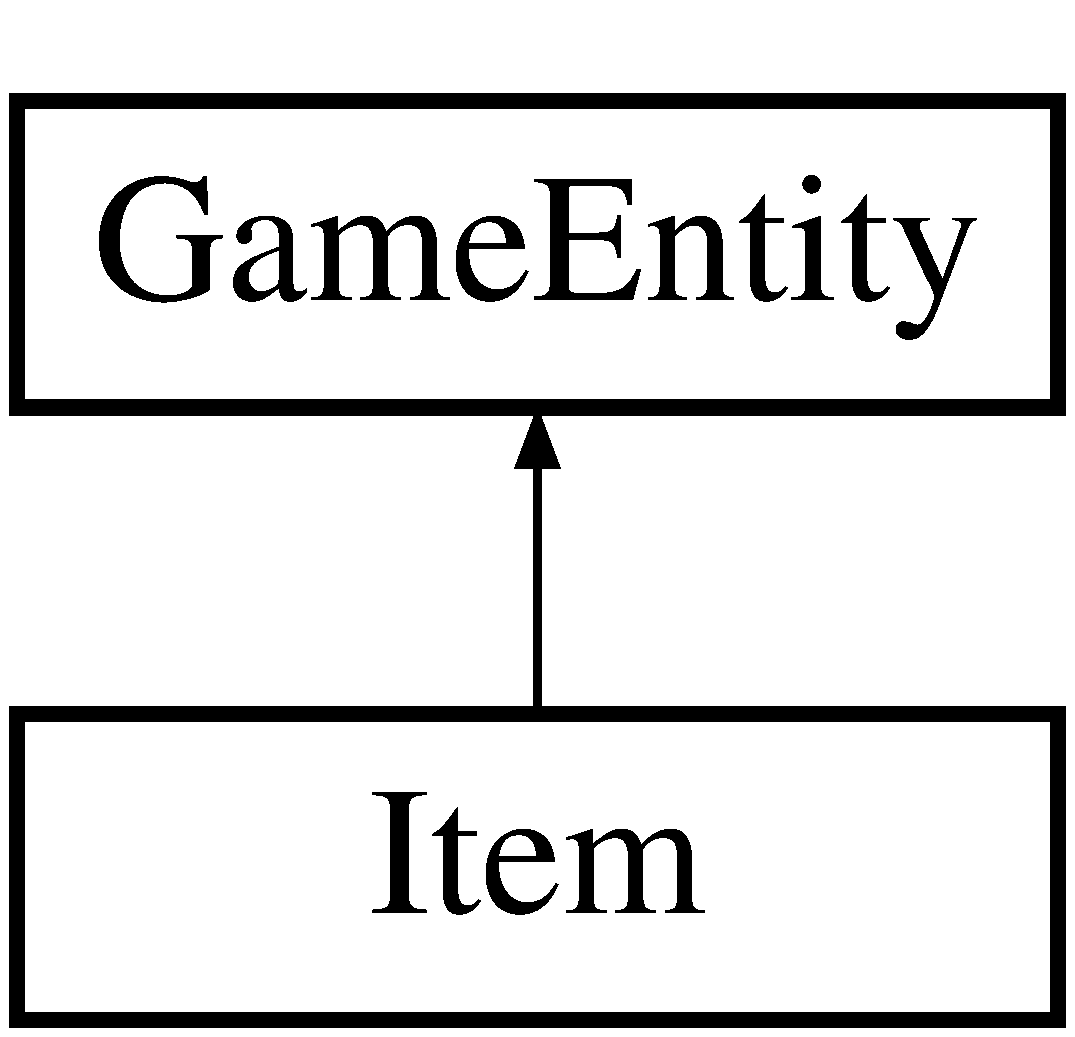
\includegraphics[height=2.000000cm]{class_item}
\end{center}
\end{figure}
\subsection*{Public Member Functions}
\begin{DoxyCompactItemize}
\item 
\hypertarget{class_item_a5ff2353dcd5cb6808c7cc101bc07cef3}{}\hyperlink{class_item}{Item} $\ast$ {\bfseries Clone} ()\label{class_item_a5ff2353dcd5cb6808c7cc101bc07cef3}

\item 
\hypertarget{class_item_a1de089cb4e92ab58a297c442c69109be}{}{\bfseries Item} (int id, std\+::string description)\label{class_item_a1de089cb4e92ab58a297c442c69109be}

\item 
\hypertarget{class_item_a7fc39ba8739faa4ea1bd60f1863f770b}{}{\bfseries Item} (int id, std\+::string name, std\+::string description)\label{class_item_a7fc39ba8739faa4ea1bd60f1863f770b}

\end{DoxyCompactItemize}


The documentation for this class was generated from the following files\+:\begin{DoxyCompactItemize}
\item 
/\+Users/\+Christina\+G/\+C\+S\+C/seng330/project/temp/temp2/Item.\+h\item 
/\+Users/\+Christina\+G/\+C\+S\+C/seng330/project/temp/temp2/Game\+Entity.\+cpp\end{DoxyCompactItemize}

\hypertarget{class_room}{}\section{Room Class Reference}
\label{class_room}\index{Room@{Room}}
Inheritance diagram for Room\+:\begin{figure}[H]
\begin{center}
\leavevmode
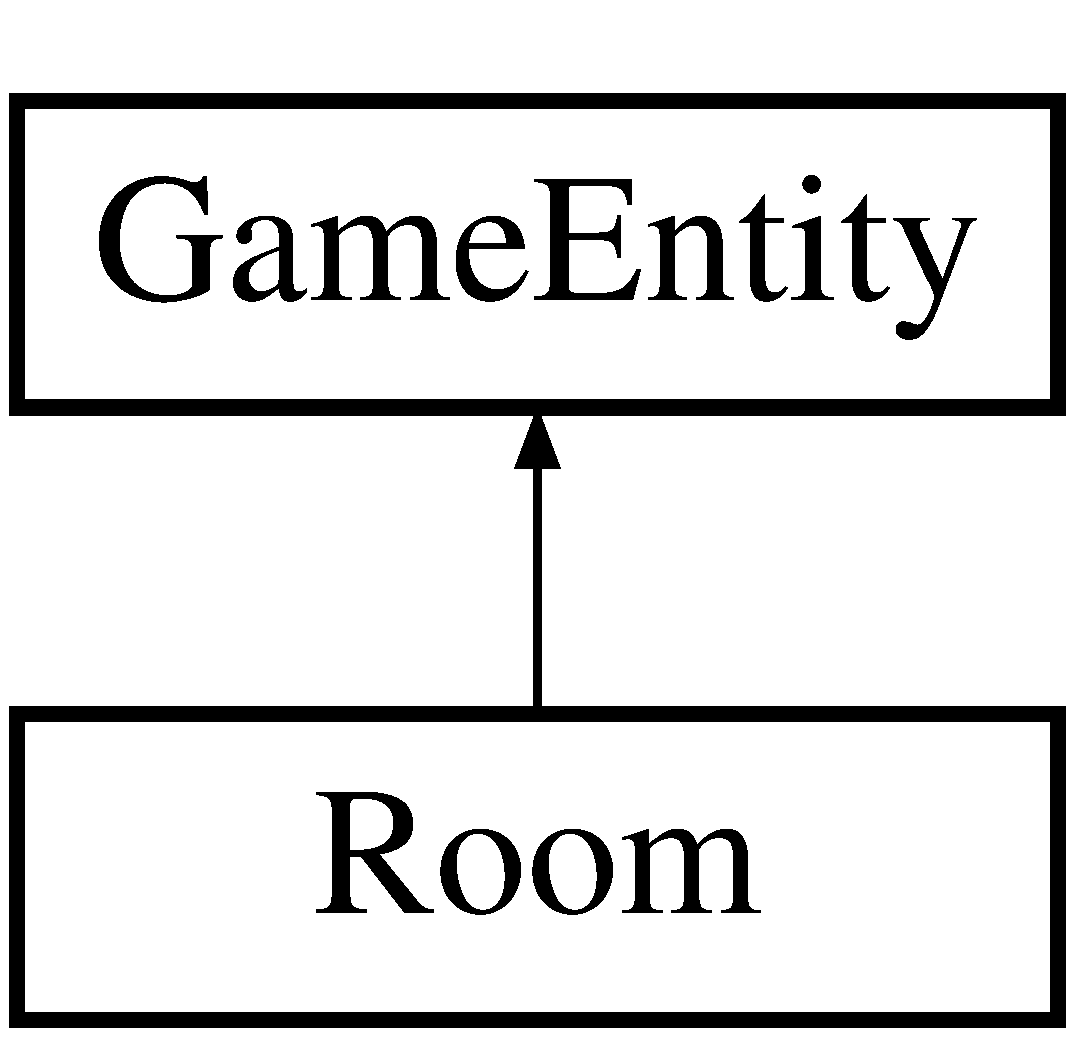
\includegraphics[height=2.000000cm]{class_room}
\end{center}
\end{figure}
\subsection*{Public Member Functions}
\begin{DoxyCompactItemize}
\item 
\hypertarget{class_room_a15e3463eb05ec8de060d67fb11f6688d}{}\hyperlink{class_room}{Room} $\ast$ {\bfseries Clone} ()\label{class_room_a15e3463eb05ec8de060d67fb11f6688d}

\item 
\hypertarget{class_room_a18d9c7ed056c4bec868cf6939dc90aac}{}{\bfseries Room} (int id, std\+::string name)\label{class_room_a18d9c7ed056c4bec868cf6939dc90aac}

\item 
\hypertarget{class_room_a2286569deae9af3cafc5716ce72dcbf1}{}{\bfseries Room} (int id, std\+::string name, std\+::string description)\label{class_room_a2286569deae9af3cafc5716ce72dcbf1}

\end{DoxyCompactItemize}


The documentation for this class was generated from the following files\+:\begin{DoxyCompactItemize}
\item 
/\+Users/\+Christina\+G/\+C\+S\+C/seng330/project/temp/temp2/Room.\+h\item 
/\+Users/\+Christina\+G/\+C\+S\+C/seng330/project/temp/temp2/Game\+Entity.\+cpp\end{DoxyCompactItemize}

%--- End generated contents ---

% Index
\backmatter
\newpage
\phantomsection
\clearemptydoublepage
\addcontentsline{toc}{chapter}{Index}
\printindex

\end{document}
